\chapter{Nowa metoda oceny procesu gojenia ścięgna Achillesa}
\label{NewMethod}

%ATRS \cite{Kearney2012}, VISA-A \cite{Robinson2001} or FAOS \cite{Roos2001} - dorzuć do biomechaniki.

%	Medical Imaging - especially Magnetic Resonance Imaging (MRI) and Ultrasonography (US) - is one of the most common technique that nowadays is used to monitor soft tissues. Some papers e.g.  \cite{Khan2003, Ibrahim2013} indicate the advantage of MRI over US showing that MRI appearance can be easier associated with the clinical outcomes. Despite this, US also present in e.g. \cite{vanSchie2009, PradoCosta2018} as a valuable technique for the soft tissues properties investigation, yet technical issues and lack of standardization limits its use.} - dorzuć do USG/MRI

W tym rozdziale zostanie zaprezentowana autorska propozycja metody oceny procesu gojenia się ścięgna Achillesa bazująca na badaniach obrazowych. W szczególności przedstawiony zostanie ilościowy opis, umożliwiający w zobiektywizowany sposób ocenę morfologii tkanek widocznych w obrazach Rezonansu Magnetycznego i Ultrasonografii. Finalnie zostanie również zaproponowane nowatorskie podejście do automatycznego wyliczania wskazanych w opisie procesu parametrów, co jest najważniejszym osiągnięciem całości tej pracy. 

Wskazana automatyzacja została przez autora wykonana dla danych z Rezonansu Magnetycznego, które zostały przez specjalistów wskazane jako klinicznie bardziej istotne niż USG. Niemniej jednak dane Ultrasonografii zostały również przeanalizowane pod kątem wartości dodanej do całego proponowanego procesu.  

W chwili pisania tej pracy nie istnieje wedle najlepszej wiedzy autora podejście umożliwiające zobiektywizowany i co ważniejsze automatyczny sposób oceny badań obrazowych prezentujących gojące się ścięgno Achillesa. Stąd implikacje dotyczące trudności z integracją subiektywnych interpretacji ze skalami testów funkcjonalnych takich jak ATRS i w rezultacie zmniejszona efektywność całego procesu oceny rehabilitacji. 

Podczas próby rozwiązania wskazanego problemu autor tej pracy w szczególności chce skupić się na dwóch aspektach. Pierwszym z nich jest jakość generowanej automatycznie oceny odniesiony do jakości wzorca tj. oceny doświadczonego radiologa. Drugim natomiast jest czas akwizycji danych, a zatem wybór praktycznego protokołu, który zapewni możliwie krótki udział pacjenta w badaniu. W obu przypadkach celem jest poszukiwanie punktu optimum, w którym maksymalizowana będzie jakość oceny, a minimalizowany czas, zarówno radiologa jak i pacjenta, niezbędny do wykonania koniecznych czynności. Szczegóły podejścia zostały opisane w kolejnej sekcji.

   

%\textcolor{blue}{The perturbations in the healing process of the Achilles tendon may result from the surgery, further rehabilitation and other factors like diet, obedience to treatment guidelines and patient predispositions. Thus, challenges in the assessment process are connected to the proper recognition of the morphological changes of the tendon structure, its functional limitations, and individual features.}

%\textcolor{blue}{


%\textcolor{blue}{Particularly there is no structured description that could apply to MRI and US studies of the Achilles tendon. The existing approaches like ATRS  \cite{Kearney2012}, VISA-A \cite{Robinson2001} or FAOS \cite{Roos2001} are only suitable for measuring the general outcome, related to symptoms and physical activity of patients. The motivation for our work is to utilize medical imaging techniques to improve precise monitoring and comparison of different therapies for ruptured Achilles tendon.}

%\textcolor{blue}{Thus we performed a broad study on 60 patients who underwent the open surgical reconstruction. The patients were monitored over a year of rehabilitation with the use of 10 MRI and 2 US protocols, acquired in 10 properly distributed time-steps. We also gathered a homogeneous control group composed of 29 healthy volunteers. To our best knowledge, there is no such study comparable in scale to the one that we introduce in this paper. For example, in\cite{Tam2017} the conclusions are formulated based on two samples, in \cite{Fujikawa2007} the authors evaluate a total of 30 healing tendons repaired with a percutaneous surgical technique and 10 repaired with an open surgical one, finally in \cite{Albano2017} the authors present results for 43 patients to study the significance of growth factors.}


\section{Metodyka}

W tej sekcji zostanie szczegółowo opisana proponowana metoda automatycznej oceny procesu gojenia się ścięgna Achillesa widocznego w badaniach obrazowych Rezonansu Magnetycznego. Dodatkowo scharakteryzowany zostanie zbiór danych, który posłużył do opracowania rozwiązania, jak również ankieta walidacyjna stanowiąca wzorzec odniesienia dla przedstawionej metody. 

Autor tej pracy, w proponowanym podejściu skorzystał z metod widzenia komputowego, a dokładniej z fuzji algorytmów sztucznej inteligencji i przetwarzania obrazów. W kontekście tej pracy, pierwsze znajdują swoje zastosowanie do ekstrakcji wektora cech dla danej reprezentacji obrazowej. Drugie, pozwalają uwzględnić wiedzę dziedzinową w procesie numerycznej oceny.

W przypadku algorytmów sztucznej inteligencji zastosowano  opisane w Rozdziale \ref{CNNs} konwolucyjne sieci neuronowe, a dokładniej AlexNet, GoogLeNet (inceptionV3) i ResNet-18. W pierwszej kolejności wykonane zostało szkolenie podanych sieci dla problemu binarnej klasyfikacji tj. odróżniania obrazów chorego od zdrowego ścięgna. Następnie część klasyfikująca została usunięta z topologii sieci, pozostawiając ekstraktor cech z parametrami zoptymalizowanymi pod kątem wydobycia istotnej informacji opisującej różnice między zdrową i chorą tkanką. Na tak otrzymanym wektorze, przeprowadzono redukcję wymiarowości z wykorzystaniem metody PCA (zob. \ref{DimReduction}). W wyniku przeprowadzonych eksperymentów, ostatecznie zdecydowano się uwzględnić 200 pierwszych czynników głównych w końcowym rozwiązaniu.

W przypadku metod przetwarzania obrazów zastosowano obliczenia cech z wydzielonego przez specjalistę radiologa ROI (od ang. \textit{Region of Interest}) reprezentującego tkanki otoczone ościęgnem. Sumarycznie wyliczono 46 klasycznych cech obrazowych, w tym pole powierzchni ROI, 9 cech opisujących statystykę wartości pikseli i 36 cechy Haralick'a opisujące teksturę (zob. \cite{Haralick1973}). W ramach statystyk scharakteryzowano: min, max, średnią, odchylenie standardowe, skośność, kurtozę, 25-percentyl, medianę oraz 75-percentyl. Natomiast w ramach cech Haralick'a: drugi moment kątowy, kontrast, korelacja, wariancja, odwrotny moment różnicowy, suma średnich, suma wariancji, suma entropii, entropia, różnica wariancji i maksimum prawdopodobieństwa. Cechy Haralick'a wyliczono dla 3 dystansów separacji \textit{d}=1,5,10. Dokładna metoda selekcji powyższych cech została przedstawiona w pracy  \cite{Nowosielski17}.  

Spośród tak wyliczonych 246 cech dokonano selekcji metodą LASSO (zob. [opis]). W rezultacie dla wszystkich ocenianych parametrów uzyskano optymalną mieszaninę poniżej 20 cech ekstrahowanych z wykorzystaniem sieci konwolucyjnych oraz klasycznych metod obrazowych. Wybrane predyktory posłużyły do szkolenia algorytmu meta-regresji, przy użyciu którego wykonana została fuzja.   

Końcowa ocena badania została wykonana następującą metryką $H$ zaproponowaną przez autora tej pracy:
\begin{equation}
H = TM(R(x_1), R(x_2),..., R(x_n))
\end{equation}
gdzie $TM$ jest średnią trymowaną z marginesami 2.5\%, a $R(x_i)$ jest wynikiem regresji obliczonym dla przekroju osiowego $x_i$, gdzie $i$ to indeks przekroju w trójwymiarowym badaniu RM.

Schemat powyższej metody został zaprezentowany na Fig. \ref{fig:net}. 
\begin{figure}[h!]
	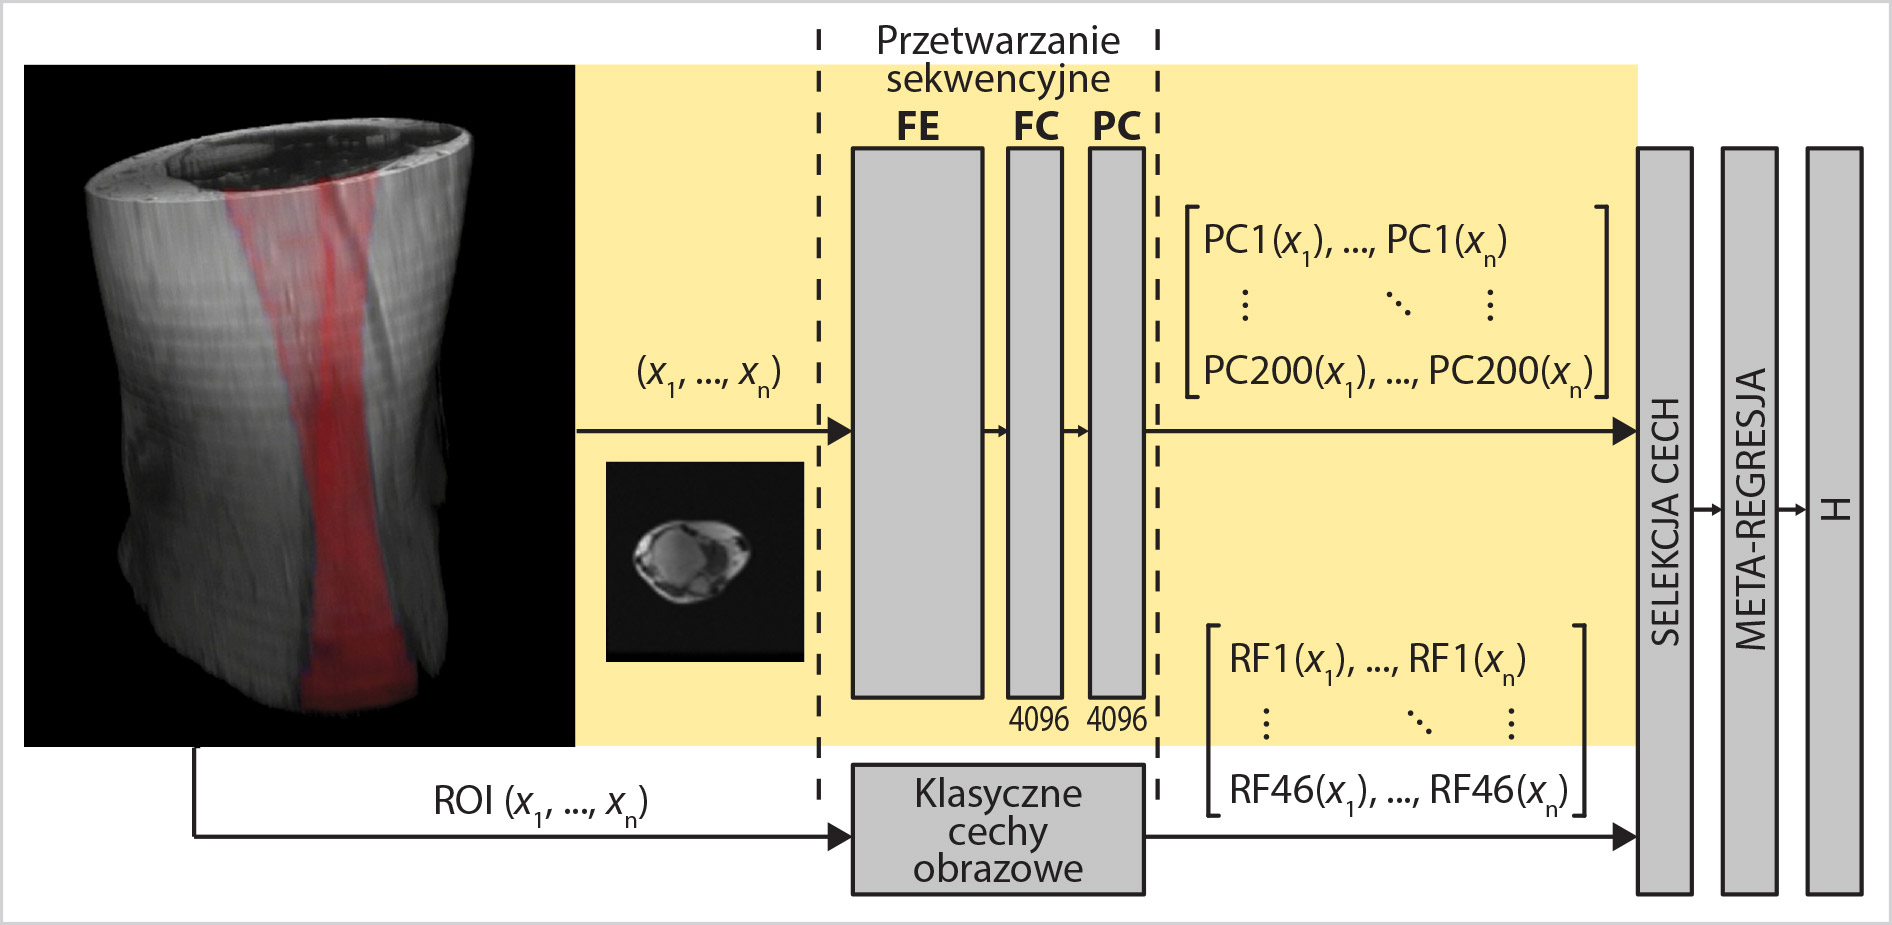
\includegraphics[width=\textwidth]{figures/net.jpg}
	\caption{Schemat automatycznej metody oceny procesu gojenia się ścięgna Achillesa.} \label{fig:net}
\end{figure}
W ogólnym ujęciu trójwymiarowe badanie RM dzielone jest na pojedyncze przekroje osiowe, które stanowią dane wejściowe do oznaczonej na żółto części opartej o metody głębokiego uczenia się. Początkowo dane przetwarzane są prze ekstraktor cech sieci AlexNet wybranej w wyniku eksperymentów (FE). Następnie wstępnie grupowane są z wykorzystaniem warstwy fully connected (FC) i poddane redukcji z 4096 pojedynczych wyjść aktywacyjnych do 200 czynników głównych (PC).

Równolegle, ROI z każdego z przekrojów stanowi dane wejściowe do części obliczeń klasycznych cech obrazowych. Końcowa fuzja wyselekcjonowanych cech z wykorzystaniem meta-regresji i metryki $H$ zapewnia numeryczny opis składający się z pojedynczej wartości dla całego badania RM w każdym z ocenianych parametrów.

\subsection{zbiór danych}
\subsection{wzorzec odniesienia}

\section{Rozróżnienie ścięgna zdrowego i po zerwaniu}
\section{Obliczanie krzywych gojenia}
\begin{equation}
H = \alpha + \sum_{i=1}^{3}\beta_{i}X_{i} + \sum_{i=1}^{3}\gamma_{i}X_{i}^{2} +
\sum_{\substack{i, j = 1\\ i < j}}^{3}\lambda_{i,j}X_{i}X_{j}
\end{equation}

gdzie $X_i = TM(PC_n(x_1), PC_n(x_2),..., PC_n(x_n))_{i}$ to kolejne predyktory, $TM$ to średnia trymowana z marginesami 2.5\%, $PC_n(x_k)$ to $n$-ty czynnik główny otrzymany przy wnioskowaniu sieci dla przekroju osiowego $x_k$, gdzie $k$ jest indeksem przekroju danego protokołu w trójwymiarowym badaniu RM.

\subsection{Topologia sieci}
\subsection{Redukcja wymiarowości}
\subsection{Miara wygojenia}
